%%%%%%%%%%%%%%%%%%%%%%%%%%%%%%%%%%%%%%%%%%%%%%%%%%%%%%%%%%%%%%%%%
%                                                               %
%        NamedGraphs       encodage : utf8                      %
%                                                               %
%%%%%%%%%%%%%%%%%%%%%%%%%%%%%%%%%%%%%%%%%%%%%%%%%%%%%%%%%%%%%%%%%
%                                                               %
%           Créé par Alain Matthes le 14/03/2007                %
%  Copyright (c) 2007 __Collège Sévigné__ All rights reserved.  %
%        version : 1.0                                          %
%%%%%%%%%%%%%%%%%%%%%%%%%%%%%%%%%%%%%%%%%%%%%%%%%%%%%%%%%%%%%%%%%
% This file may be distributed and/or modified
%
% 1. under the LaTeX Project Public License , either version 1.3
% of this license or (at your option) any later version and/or
% 2. under the GNU Public License.
% See http://www.latex-project.org/lppl.txt for details.    
% graphs from graph theory

\documentclass[DIV         = 12,
               fontsize    = 10,
               headinclude = false,
               index       = totoc,
               footinclude = false,
               twoside,
               headings    = small
               ]{tkz-doc}  
%\usepackage{svn-multi} 
\usepackage{tkz-berge} 

\usepackage[pdftex,
            unicode,
            colorlinks    = true,
            pdfpagelabels, 
            urlcolor      = blue,
            filecolor     = pdffilecolor,
            linkcolor     = blue,
            breaklinks    = false,
            hyperfootnotes= false,
            bookmarks     = false,
            bookmarksopen = false, 
            linktocpage   = true,
            pdfsubject    ={Graph Theory},
            pdfauthor     ={Alain Matthes},
            pdftitle      ={NamedGraphs},
            pdfkeywords   ={graph,berge},
            pdfcreator    ={pdfeTeX}
            ]{hyperref}    
\usepackage{url}
\def\UrlFont{\small\ttfamily}
\usepackage[protrusion = true,
            expansion,
            final,
            verbose    = false
            ]{microtype}

\DisableLigatures{encoding = T1, family = tt*} 
  
\usepackage[parfill]{parskip}
\gdef\nameofpack{tkz-kiviat}
\gdef\versionofpack{v 1.00 c}
\gdef\dateofpack{2011/06/07}
\gdef\nameofdoc{tkz-kiviat}
\gdef\dateofdoc{2011/06/07}
\gdef\authorofpack{Alain Matthes}
\gdef\adressofauthor{}
\gdef\namecollection{AlterMundus}
\gdef\urlauthor{http://altermundus.fr}
\gdef\urlauthorcom{http://altermundus.com}
\title{The package : tkz-kiviat}
\author{Alain Matthes}
   
\usepackage{shortvrb,fancyvrb}    
\usepackage{tkzexample,tkz-kiviat}   
\makeatletter
\renewcommand*\l@subsubsection{\bprot@dottedtocline{3}{3.8em}{4.2em}}
\makeatother
\AtBeginDocument{\MakeShortVerb{\|}}

\pdfcompresslevel=9
\pdfinfo{
    /Title (tkz-kiviat.pdf)
    /Creator (TeX)
    /Producer (pdfeTeX)
    /Author (Alain Matthes)
    /CreationDate (07 juin 2011)
    /Subject (Named Graphs)
    /Keywords (pdfeTeX,  kiviat, graph, berge, tikz, pdflatex) } 
    
\usepackage{pgfplotstable}               
\usepackage[english]{babel}
\usepackage[autolanguage]{numprint}  


\begin{document}
\parindent=0pt   
\title{\nameofpack}
\date{\today}

\clearpage
\thispagestyle{empty}
\maketitle

\clearpage
\tkzSetUpColors[background=fondpaille,text=Maroon]   
\colorlet{textcodecolor}{Maroon} 
\pagecolor{fondpaille} 
\color{Maroon}   
\colorlet{graphicbackground}{fondpaille}
\colorlet{codebackground}{Peach!30}
\colorlet{codeonlybackground}{Peach!30}   


\nameoffile{\nameofpack} 

\defoffile{\textbf{tkz-kiviat.sty} is a simple package to draw Kiviat's graph with \TIKZ. Il est nécessaire d'utiliser \PGF\ 2.1. 
}
 % A lot of references can be found here  \url{http://mathworld.wolfram.com}      
\presentation

\vspace*{12pt}   

\tkzHand Firstly, I would like to thank \textbf{Till Tantau} for the  beautiful LATEX package, namely TikZ.

\vspace*{12pt}   
\tkzHand I am grateful to  \textbf{Michel Bovani} for providing the \tkzname{fourier} font.




\vspace*{12pt}
\tkzHand Vous trouverez de nombreux exemples sur mes sites~: 
\href{http://altermundus.com/pages/download.html}{altermundus.com} ou 
\href{http://altermundus.fr/pages/download.html}{altermundus.fr}    

\vfill   
Vous pouvez envoyer vos remarques, et les rapports sur des erreurs que vous aurez constatées à l'adresse suivante~: \href{mailto:al.ma@mac.com}{\textcolor{blue}{Alain Matthes}}.
 
This file can be redistributed and/or modified under the terms of the LATEX 
Project Public License Distributed from CTAN archives in directory \url{CTAN://macros/latex/base/lppl.txt}.    



\clearpage
\tableofcontents
 
\clearpage\newpage 
   
\setlength{\parskip}{1ex plus 0.5ex minus 0.2ex}
     


\newpage\section{Kiviat Graph}
\subsection{Caractéristiques d'un diagrame de Kiviat } 
La macro suivante permet de définir les caractéristiques du diagramme. En arguments est donné une liste de variables. Cette liste va déterminer le nombre d'axes radiaux. En option, vous pouvez régler le nombre de lattes formant le treillis, ainsi que d'autres options. 

\bigskip
\begin{NewMacroBox}{tkzKiviatDiagram}{\oarg{options}\var{Liste de modalités}} 
  L'argument est une liste de variables et cet argument est obligatoire.
  
\medskip
\begin{tabular}{lll}
Arguments & ex & définition                              \\ 
\midrule
\TAline{Liste de variables} {empty}  {\{charbon, gaz,uranium\}}   
\end{tabular} 

\medskip
\begin{tabular}{lll}
Options & défaut & définition               \\
\midrule
\TOline{lattice}      {10}  {nombre de lattes}
\TOline{gap}          {0.5} {l'écart entre deux lattes est de $0.5$ cm}
\TOline{space}        {0.5} {les axes sont agrandis de $0,5$ cm} 
\TOline{label space}  {1.5} {Distance en cm entre la fin de l'axe et le label}     
\TOline{step}         {1}   {}
\TOline{radial style} {1}   {style des axes radiaux}
\TOline{label style}  {1}   {style des étiquettes (labels)}
\bottomrule
\end{tabular}

\emph{Par défaut  l'axe radial est gradué de $0$ à $1$. Entre deux graduations, l'écart est de $0.5$ cm et est déterminé par l'option \tkzname{gap}.}

\end{NewMacroBox}

\bigskip
\subsubsection{Par défaut avec trois variables} 

\begin{tkzexample}[width=8cm]
\begin{tikzpicture}[scale=.5]
   \tkzKiviatDiagram{gaz,charbon,uranium}
\end{tikzpicture}
\end{tkzexample}

\subsubsection{Par défaut, mais avec cinq variables}   
Dans cet exemple, j'utilise cinq ($5$) variables : 

  Poissons,Légumes,Viande,Lait,Pain. 
  
 La toile (treillis)  est formé de dix ($10$)  lattes.

\bigskip   
\begin{tkzexample}[code only]
\begin{tikzpicture}
   \tkzKiviatDiagram{Poissons,Légumes,Viande,Lait,Pain}
\end{tikzpicture}  
\end{tkzexample}  

   
\begin{center}
\begin{tikzpicture}
 \tkzKiviatDiagram{Lait,Pain,Poissons,Légumes,Viande}
\end{tikzpicture}  
\end{center}

\subsubsection{Option \tkzname{gap} (écart entre deux lattes)}
Ceci permet de modifier l'écart entre deux lattes. Le premier exemple va prendre moins de place avec avec un écart divisé par deux.


\begin{tkzexample}[width=9cm]
\begin{tikzpicture}
   \tkzKiviatDiagram[gap=.25,
         label space=.75]{A,B,C,D,E}
\end{tikzpicture}  
\end{tkzexample} 

\subsubsection{Option \tkzname{gap} (écart entre deux lattes)}
Ceci permet de modifier l'écart entre deux lattes. Le premier exemple va prendre moins de place avec avec un écart divisé par deux.

\begin{tkzexample}[width=7cm]
\begin{tikzpicture}
   \tkzKiviatDiagram[gap=.25]{A,B,C,D,E,F}
\end{tikzpicture}
\end{tkzexample}

\subsubsection{option \tkzname{lattice} (nombre de lattes)} 
Par défaut ce nombre est de 10 ( voir l'exemple précédent) .

\begin{tkzexample}[width=7cm]
\begin{tikzpicture}
   \tkzKiviatDiagram[lattice=5]{Poissons,Légumes,Viande,Lait,Pain}
 \end{tikzpicture}
\end{tkzexample}

\subsubsection{options \tkzname{radial  style} et \tkzname{lattice style}} 
 \begin{tkzexample}[]
\begin{tikzpicture}
\tkzKiviatDiagram[
     radial  style/.style ={-},
     lattice style/.style ={blue!30}]%
{A,B,C,D,E}
 \end{tikzpicture}

 \end{tkzexample}

\newpage
\subsection{Tracé d'une ligne} 
\begin{NewMacroBox}{tkzKiviatLine}{\oarg{options}\var{$v_1,v_2,\dots$}}

 L'argument est une liste de valeurs et cet argument est obligatoire. Les valeurs sont des décimaux mais si la valeur est un entier alors c'est entier correspond au rang d'une latte. La partie décimale si elle existe, précise le placement entre deux lattes sur l'axe radial.
  
\medskip
\begin{tabular}{lll}
Arguments & défaut & exemple                              \\ 
\midrule
\TAline{Liste de valeurs} {empty}  {\{4,3,2\}}   
\end{tabular} 

\medskip
\begin{tabular}{lll}
Options & défaut & définition               \\
\midrule
\TOline{fill}      {10}  {permet de colorier l'intérieur du polygone}
\TOline{opacity}   {0.5} {définit l'opacité de la surface limitée par la ligne.}
\bottomrule
\end{tabular}

\emph{Par défaut,  l'axe radial est gradué de $0$ à $10$. Entre deux graduations, l'écart est de $0.5$ cm et est déterminé par l'option \tkzname{gap}.}   

\end{NewMacroBox} 

\begin{tkzexample}[]
\begin{tikzpicture}
   \tkzKiviatDiagram[lattice=5]{A,B,C} 
     \tkzKiviatLine[thick,
                    color      = blue,
                    mark       = ball,
                    mark size  = 4pt,
                    fill       = blue!20,
                    opacity=.5](4,3,2)   
\end{tikzpicture} 
\end{tkzexample}
  
  
\subsubsection{Exemple avec deux lignes}
\begin{tkzexample}[]
\begin{tikzpicture}
 \tkzKiviatDiagram{Poissons,Légumes,Viande,Lait,Pain}
  \tkzKiviatLine[thick,
                 color=red,
                 mark=ball,
                 ball color=red,
                 mark size=4pt,opacity=.2, 
                 fill=red!20](5,9,6,8,4)
 \tkzKiviatLine[thick,
                color=blue,
                mark=ball,
                mark size=4pt,
                fill=blue!20,
                opacity=.5](4,6,6,4,3)   
\end{tikzpicture} 
\end{tkzexample}


\subsubsection{Autre exemple}     
\begin{tkzexample}[small]
\begin{tikzpicture}[label distance=.15cm]
 \tkzKiviatDiagram[radial  style/.style ={-},
                   lattice style/.style ={blue!30}]%
        {Poissons,Légumes,Viande,Lait,Pain}
 \tkzKiviatLine[thick,color=red,
                mark=ball,
                ball color=red,
                mark size=4pt,
                fill=red!20](5,9,6,8,4)
 \tkzKiviatLine[thick,color=blue,mark=ball,
                mark size=4pt,
                fill=blue!20,
                opacity=.5](9,6,8,4,5) 
\end{tikzpicture}
\end{tkzexample}
  

\newpage
 \subsection{Graduation d'un axe}  
\begin{NewMacroBox}{tkzKiviatGrad}{\oarg{options}\varp{integer}}
\begin{tabular}{lll}
Arguments & exemple & définition                              \\ 
\midrule
\TAline{integer} {empty}  {numéro de l'axe}   
\end{tabular} 

\medskip
\begin{tabular}{lll}
Options & défaut & définition               \\
\midrule
\TOline{graduation distance}{0pt}{permet de positionner les graduations}
\TOline{prefix}   {empty} {Ajoute un préfixe devant la valeur}
\TOline{suffix}   {empty} {Ajoute un suffixe devant la valeur} 
\TOline{unity}   {1} {unité choisie pour les graduations}
\bottomrule
\end{tabular} 

\emph{Voir les exemples ci-dessous pour l'utilisation de \tkzname{suffix} et \tkzname{prefix}}

\end{NewMacroBox}  

 
 \subsubsection{Exemple avec usage de \tkzname{suffix}}  
\begin{tkzexample}[]
\begin{tikzpicture}
\tkzKiviatDiagram[scale   = .6,
                  gap     = 1,  
                  lattice = 5]{%
                  McCabe,LOC,Live Variables,Halstead N,Variablenspanne}
\tkzKiviatLine[thick,color=blue,mark=none,
               fill=blue!20,opacity=.5](3,3.5,3,3.5,3)
\tkzKiviatLine[thick,color=darkgray,
               fill=green!20,opacity=.5](0.5,1,0.5,0.75,1) 
\tkzKiviatLine[ultra thick,mark=ball,
                 mark size=4pt,color =Maroon](2,3.75,1,1.5,2)    
\tkzKiviatGrad[prefix=,unity=100,suffix=\ \texteuro](1)  
\end{tikzpicture}
\end{tkzexample}
   

 \subsubsection{Autre exemple avec usage de \tkzname{prefix}}  
\begin{tkzexample}[]
\begin{tikzpicture}[rotate=30,scale=.75]
\tkzKiviatDiagram[lattice     = 6,
                  gap         = 1,
                  step        = 2,
                  label space = 2]%
       {Marketing,
        Sales,
        Administration,
        Information Technology,
        Customer Support,
        Development}
  \tkzKiviatLine[thick,color=red](2.25,2.5,0.6,1.2,1,1)
  \tkzKiviatLine[thick,color=blue](1,2,1,1.7,1.3,3)
  \tkzKiviatGrad[prefix=\$,unity=10](5)
 \end{tikzpicture}
\end{tkzexample}
  
 
 
 
\newpage\section{Kiviat Graph à l'aide d'un fichier}
Ce fichier est lu avec \tkzname{pgfplots}\NamePack{pgfplots}. 

\subsection{Caractéristiques du diagramme} 
    
\begin{NewMacroBox}{tkzKiviatDiagramFromFile}{\oarg{options}\var{file}}
Le fichier doit être un fichier correspondant aux fichiers du package \tkzNamePack{pgfplots}. 

\medskip
\begin{tabular}{lll}
Arguments & défaut & exemple                              \\ 
\midrule
\TAline{file} {empty}  {file.dat (\tkzname{pgfplots}\NamePack{pgfplots}.)}   
\end{tabular} 

\medskip
\begin{tabular}{lll}
Options & défaut & définition               \\
\midrule
\TOline{lattice}      {10}  {nombre de lattes}
\TOline{gap}          {0.5} {l'écart entre deux lattes est de $0.5$ cm}
\TOline{space}        {0.5} {les axes sont agrandis de $0,5$ cm} 
\TOline{label space}  {1.5} {Distance en cm entre la fin de l'axe et le label}     
\TOline{step}         {1}   {}
\bottomrule
\end{tabular}

\emph{Par défaut  l'axe radial est gradué de $0$ à $1$. Entre deux graduations, l'écart est de $0.5$ cm et est déterminé par l'option \tkzname{gap}.}    
\end{NewMacroBox}  

\begin{tkzltxexample}[]
%file2.dat
column1                    column2   
Reliability                6         
Usability                  4         
Timeliness                 2         
Efficiency                 3          
\end{tkzltxexample}    

\begin{tkzexample}[latex=8cm]
\begin{tikzpicture}
\tkzKiviatDiagramFromFile[
        scale=.2,
        label distance=1cm,
        gap     = 1,
        label space=5,  
        lattice = 10]{file2.dat}
   
\end{tikzpicture}  
\end{tkzexample}

\newpage
 \subsection{Tracé des lignes}  
\begin{NewMacroBox}{tkzKiviatLineFromFile}{\oarg{options}\var{file}\var{file}}

\medskip
\begin{tabular}{lll}
Arguments & défaut & exemple                              \\ 
\midrule
\TAline{file} {empty} {file.dat (nécessite \tkzname{pgfplots}\NamePack{pgfplots})} 
\end{tabular} 

\medskip
\begin{tabular}{lll}
Options & défaut & définition               \\
\midrule
\TOline{fill}      {10}  {permet de colorier l'intérieur du polygone}
\TOline{opacity}   {0.5} {définit l'opacité}
\bottomrule
\end{tabular} 

\emph{L'opacité ne pose pas de problème avec \tkzname{pdflatex} mais peut entraîner quelques difficultés avec \tkzname{latex}.}  

\end{NewMacroBox}   

\subsubsection{Diagramme à l'aide de données stockées dans un fichier}  
Ce fichier est lu à l'aide de \tkzname{pgfplots}\NamePack{pgfplots}. Voici un exemple de fichiers.

\begin{tkzltxexample}[]
 %file.dat
 column1                    column2   column3 
 Reliability                6           6.5
 Usability                  4           9
 {Application Architecture} 7           8
 {Version Control}          6.5         7
 Timeliness                 2           8
 Efficiency                 3           4
 Effectiveness              5           6.5
 Interoperability           1.5         7
\end{tkzltxexample}

\begin{tkzexample}[latex=9cm]
\begin{tikzpicture}
\tkzKiviatDiagramFromFile[
        scale          =.25,
        label distance =.5cm,
        gap            = 1,
        label space    = 4,  
        lattice        = 10]{file.dat}
\tkzKiviatLineFromFile%
  [thick,
   color      = blue,
   mark       = ball,
   ball color = blue,
   mark size  = 4pt,
   fill       = blue!20]{file.dat}{2}
\tkzKiviatLineFromFile%
   [thick,
    color      = red,
    mark       = ball,
    ball color = red,
    mark size  = 4pt,
    fill       = red!20]{file.dat}{1} 
\end{tikzpicture}
\end{tkzexample}
   

\clearpage\newpage
\printindex
\end{document}

